\documentclass[11pt,a4paper]{article}
\usepackage[margin=24mm]{geometry}
\usepackage[T1]{fontenc}
\usepackage[utf8]{inputenc}
\usepackage{lmodern}
\usepackage{graphicx}
\usepackage{booktabs}
\usepackage{longtable}
\usepackage{array}
\usepackage{listings}
\usepackage{xcolor}
\usepackage{hyperref}
\usepackage{microtype}
\usepackage{enumitem}
\usepackage{float}
\hypersetup{colorlinks=true,linkcolor=blue,urlcolor=blue}
\lstset{basicstyle=\ttfamily\small,breaklines=true,frame=single,columns=fullflexible}
\setlength{\parskip}{.55em}
\setlength{\parindent}{0pt}
\title{AMAC 3D\\A guide to metric-driven tetrahedral adaptation}
\author{}
\date{}
\begin{document}
\maketitle
\begin{abstract}
AMAC (anisotropic mesh adaptation code) adapts an existing tetrahedral mesh to a target metric field. This guide covers setup, a first run, metric generation, computer-aided design (CAD) projection, outputs and known limits.
\end{abstract}
\setcounter{tocdepth}{1}
\tableofcontents
\clearpage

\section{What AMAC does}
A metric assigns a desired spacing and direction at each point. AMAC reads a tetrahedral mesh and a metric sampled at its nodes. The engine splits long edges, collapses short edges, reconnects local tets and smooths nodes.

AMAC repeats these steps in four groups, called the ABCD cycle. The run ends at its iteration cap or when its edge-length extremes stabilize. AMAC writes a mesh after each iteration and a final visualization mesh.

An isotropic metric requests the same spacing in every direction. An anisotropic metric can ask for fine resolution across a feature and larger cells along it. AMAC stores a symmetric tensor with six components per node. An edge conforms when its metric length lies between $1/\sqrt2$ and $\sqrt2$. Boundary and quality constraints can leave some edges outside this target band.

AMAC needs an initial mesh. The bundled cube cases supply one. Optional pyEGADS support projects boundary nodes to a STEP model. The analytical geometry reader handles planes and spheres without it.

AMAC runs in one process with Numba kernels and Threading Building Blocks (TBB) threads. The public case runner is \texttt{run/adapt.py}. Its case files are in \texttt{cases/}.

Figure~\ref{fig:caseflow} shows the interaction between a case file, the driver and the engine. Validation happens before the engine starts. You can stop at the resolved-case report with \texttt{--check}, or let the driver build the two grids and run adaptation.
\begin{figure}[H]
\centering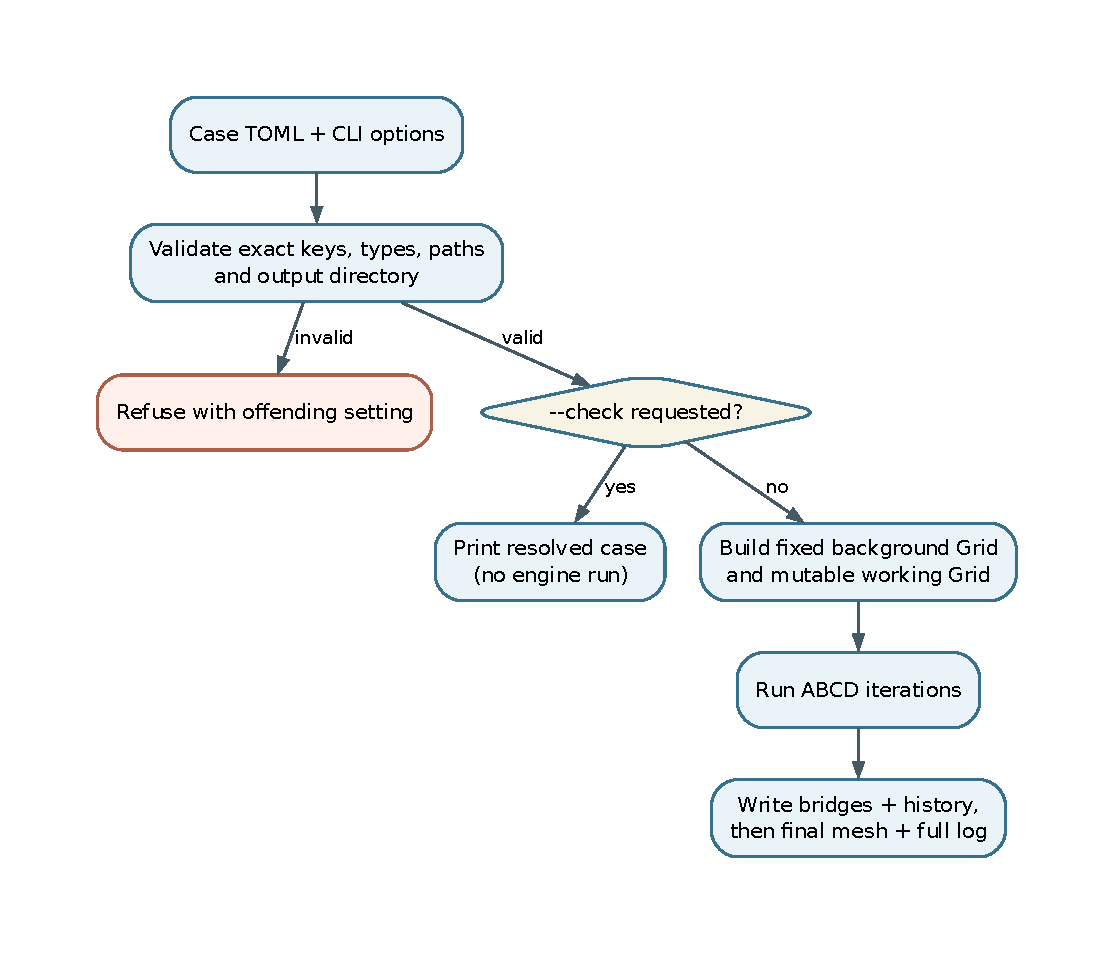
\includegraphics[width=.95\linewidth]{docs/figures/case_to_mesh.pdf}
\caption{From a case file to mesh outputs. The refusal path names the invalid setting; the check path does not start adaptation. A normal run uses a fixed background grid and a mutable working grid.}
\label{fig:caseflow}
\end{figure}

\section{Install and activate}
Run the setup script from the repository root with a supported Python interpreter on your path:
\begin{lstlisting}[language=bash]
bash setup.sh
source activate.sh
\end{lstlisting}
The setup script creates \texttt{.venv}, installs the pinned Python packages, checks TBB, and runs the short regression lane. Source \texttt{activate.sh} in every new shell before using the driver or tools. It selects the project interpreter, sets the package path, and checks the Numba threading layer before changing the shell environment. The activation message prints the interpreter and TBB library it selected.

For STEP projection, install the optional ESP/pyEGADS support, then activate again:
\begin{lstlisting}[language=bash]
bash setup.sh --esp
source activate.sh
\end{lstlisting}
\texttt{setup.sh --force --esp} obtains a fresh ESP archive. \texttt{setup.sh --clean} lists the paths it would remove; \texttt{--yes} confirms that cleanup. A basic cube case does not require ESP.

\section{Quick start: the cross metric}
First inspect the bundled case without starting adaptation:
\begin{lstlisting}[language=bash]
source activate.sh
python -m run.adapt cases/cube_cross/case.toml --check
\end{lstlisting}
The command prints resolved absolute input paths, settings, an output path, and the engine commit when Git can identify it. It checks the schema and verifies that each input file exists. The dry check is a useful first step after moving a case file or changing an output directory.

To run the case, choose a result directory that is separate from \texttt{input/}:
\begin{lstlisting}[language=bash]
python -m run.adapt cases/cube_cross/case.toml --iterations 12 --threads 4 --output-dir /tmp/amac-cube-cross
\end{lstlisting}
This run can take time. The console shows the input names, one line per completed iteration, a stop reason, and the files written. The chosen directory receives the full time-stamped log. If that directory already contains files, choose a new one or pass \texttt{--force} after checking its contents. Keep \texttt{resolved\_case.json} with any quality figure you report: it records the effective settings and provenance.

The second bundled cross case, \texttt{cases/cube\_cross\_coarse/case.toml}, uses a coarser metric. \texttt{cases/cube\_cylinder/case.toml} uses a cylinder field. Each case keeps its geometry, mesh and metric under its own \texttt{input/} directory so a case can be copied without changing paths.

\clearpage
\section{A STEP-backed case}
After installing optional ESP support, inspect the CAD case:
\begin{lstlisting}[language=bash]
source activate.sh
python -m run.adapt cases/cube_egads/case.toml --check
python -m run.adapt cases/cube_egads/case.toml --threads 4 --output-dir /tmp/amac-cube-egads
\end{lstlisting}
The case pairs \texttt{cube.step} with an initial Netgen mesh and a \texttt{.geo} description. The STEP model supplies exact boundary projection where pyEGADS can map a face or edge. The mesh still supplies the starting tetrahedra and boundary tags. A STEP file alone is not an initial volume mesh.

The adapter accepts one CAD body. If pyEGADS is absent, activation reports that optional support is unavailable. Install it before running this case. Without a STEP model, the \texttt{.geo} reader projects onto recognized planes and spheres. Other curved boundaries use a mesh-based fallback, which can have larger geometric error.

\section{Generate a metric}
The bundled generator can sample an analytic field at the vertices of a Netgen \texttt{.vol} mesh. It knows the \texttt{cross}, \texttt{cylinder}, and \texttt{uniform} fields. List the registered names and parameters before choosing values:
\begin{lstlisting}[language=bash]
source activate.sh
python tools/analytic_metric_generator.py list
python tools/analytic_metric_generator.py generate --mesh cases/cube_cross/input/mesh/cube1241.vol --metric cross --param scale=0.2 --output cross_custom.sol --output-dir /tmp/amac-metrics
\end{lstlisting}
The generator writes one six-component symmetric tensor per mesh node in Medit \texttt{.sol} format. Paths under \texttt{[input]} resolve from the case file unless they are absolute. Add the generated metric path there.

A metric must have positive eigenvalues. Check the node count and component order when another program writes the metric. The supplied cylinder metric is a fixed input; current generator defaults do not recreate it. Record parameters whenever you generate a replacement.

\subsection{Check a field before using it}
The generator can compare an analytic field with a reference metric at the same mesh points. This check is useful when you copy a case metric or change a formula:
\begin{lstlisting}[language=bash]
python tools/analytic_metric_generator.py validate --mesh cases/cube_cross/input/mesh/cube1241.vol --metric cross --reference cases/cube_cross/input/metric/cross.sol
\end{lstlisting}
The report gives relative error and can list the worst nodes with \texttt{--verbose}. Pass \texttt{--tolerance} to make a larger error fail the command. A mismatch can come from different field parameters, point ordering, or a component-order convention. The generator accepts repeated \texttt{--param} assignments, so a validation command should record them in the same way as the generation command.

The six tensor entries are the upper triangle in the order $M_{11},M_{12},M_{13},M_{22},M_{23},M_{33}$. An external Medit writer may use another order. Reconstruct one anisotropic $3\times3$ matrix and check its eigenvalues before loading the field. An isotropic test, $M=h^{-2}I$, checks spacing and units.

AMAC interpolates matrix logarithms to preserve positive definiteness. Arithmetic averaging of tensor entries can change target edge lengths.

The background field and working mesh have different jobs. \texttt{mesh\_prev} and its \texttt{metric} define a fixed sampled field. \texttt{mesh} supplies the elements that operators change. On a newly split edge or an accepted smooth move, the working grid samples the background field at the new position. This design lets you restart from a different working mesh while retaining the same target field, provided the background mesh covers the positions you query. A point outside that background can make field lookup fail; verify domains before a long run.

\section{The case file and driver policy}
A case has three tables. The example shows the four file inputs and the settings most users change:
\begin{lstlisting}
[input]
geometry = "input/geometry/cube.geo"
mesh_prev = "input/mesh/cube1241.vol"
mesh = "input/mesh/cube1241.vol"
metric = "input/metric/cross.sol"

[adapt]
iterations = 20
enable_swap = true

[run]
output_dir = "output"
output_name = "cube_cross_adapted"
output_format = "vtk"
\end{lstlisting}
The background mesh \texttt{mesh\_prev} carries the sampled metric. The working \texttt{mesh} is the starting topology that AMAC changes. They may be the same file, as in the bundled cube. Add \texttt{egads = "input/geometry/cube.step"} under \texttt{[input]} for CAD projection. The reference manual shipped with the source lists every key, type, default and allowed value.

All four bundled cases use this three-table schema. A missing key takes its loader default. You can also choose the bridge format, collapse sweep cap, rejection detail, final mesh format and log name. The reference manual lists every key, default and allowed value.

The loader accepts exact known keys only. It names an unknown table or key, wrong type, unsupported format, missing input or out-of-range count. It refuses output inside any \texttt{input/} directory. It also refuses an existing nonempty result directory unless you pass \texttt{--force}.

Thread count stays on the command line. The case file has no keys for worker count, threading layer, kernel choices, tolerances or quality thresholds. The engine owns those settings. Add a case key only when users need it and its default reproduces the reference cases.

\clearpage
\subsection{Inside one adaptation iteration}
The engine follows the sequence in Figure~\ref{fig:cycle}. A coarsens, B smooths, C refines, and D smooths again. The engine then checks for flat tetrahedra, writes the iteration mesh and history, and decides whether another cycle is needed. The iteration limit caps that loop; stable edge-length extremes can end it earlier.
\begin{figure}[H]
\centering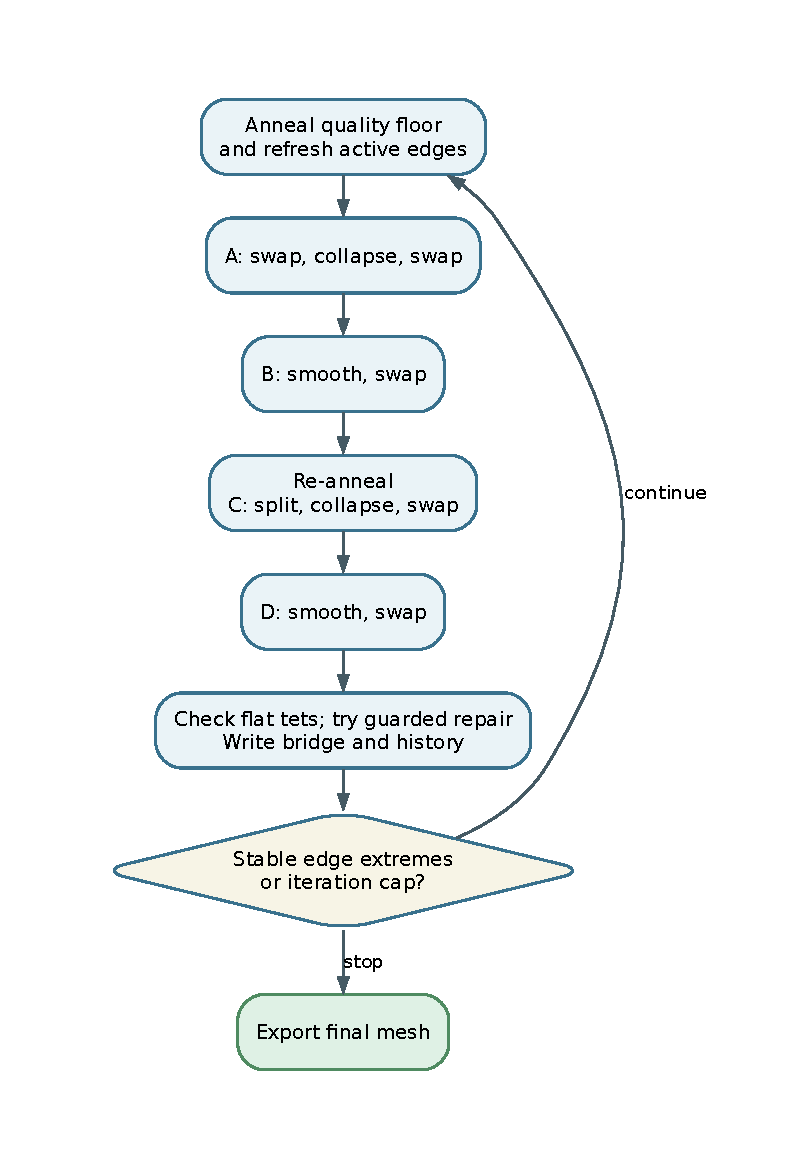
\includegraphics[height=.70\textheight,keepaspectratio]{docs/figures/abcd_cycle.pdf}
\caption{One ABCD cycle and the stop decision. Each attempted local change passes the applicable boundary, signed-volume, quality and collision checks before the engine commits it. The pure-interior collapse path uses its documented intersection exemption.}
\label{fig:cycle}
\end{figure}

\clearpage
\section{Control and read output}
\texttt{[run].output\_dir} defaults to \texttt{output} beside the case file. A relative value resolves there; an absolute value stays absolute. \texttt{--output-dir} overrides the file. Use a fresh directory for each comparison so the result and its resolved settings remain together. A normal run writes the following files:

\begin{longtable}{>{\ttfamily}p{.37\linewidth}p{.55\linewidth}}
\toprule
\normalfont File & Meaning\\
\midrule
\endhead
resolved\_case.json & Absolute inputs, effective options, thread count, output path, engine commit.\\
adaptation.log & Full engine messages and timestamps, including details suppressed on the console.\\
bridge\_i.msh & Mesh after iteration $i$, starting at zero. The case can select \texttt{vol} or both bridge formats.\\
adaptation\_history.json & Per-iteration node and tet counts, metric edge lengths, quality and complexity statistics, with stopping information.\\
cube\_cross\_adapted.vtk & Final visualization mesh for the bundled cross case. The case can request \texttt{msh} or both final formats.\\
\bottomrule
\end{longtable}

The console presents a compact progress table; read the full log when a pass rejects candidates or a run stops unexpectedly. A maximum dihedral angle appears in the final display in degrees. The JSON history keeps its established fields; the display value does not add a new history key. Bridge meshes use Gmsh 2.2 ASCII by default, while a final VTK file is intended for visualization.

\subsection{Interpret the progress numbers}
The edge-length summary measures the mesh in its target metric. The conforming percentage counts edges between $1/\sqrt2$ and $\sqrt2$; it is a fraction, not a proof that every element is valid. Compare the minimum and maximum lengths to see whether extreme short or long edges remain. A changing mesh can improve the conforming fraction while some constrained boundary edges stay outside the band.

The Knupp quality $Q$ summarizes tetrahedron shape in the metric. A regular isotropic tet scores one, and a flat tet scores zero. Mean $Q$ describes the mesh as a whole. The minimum and the count below a small threshold expose poor cells.

The formula gives an inverted tet the same score as its reversed counterpart. AMAC therefore checks signed volume before accepting an operation. If a solver is sensitive to isolated bad cells, inspect the final mesh even when the flat count is zero.

Complexity estimates the node budget implied by the metric through an integral of $\sqrt{\det M}$. The history also records nodes divided by complexity. The engine reports this ratio without using it to throttle splits. A metric with larger eigenvalues usually asks for more resolution and raises complexity; the exact result still depends on boundaries and local quality gates. Compare complexity only when the input domain and metric definition are the same.

The iteration cap is a maximum. The convergence test can stop earlier after the minimum and maximum metric edge lengths stabilize. The final report gives the stop reason. For comparisons, record both the cap and the completed iteration count. Two runs with the same cap can stop at different times.

\clearpage
\section{Inspect and convert a mesh}
\subsection{Metric and angle histograms}
\texttt{tools/analyze\_mesh.py} measures physical and metric dihedral angles and metric edge lengths. Use a mesh and metric sampled on matching node sets; pass \texttt{--bg-mesh} when the metric belongs to a separate background mesh. Direct its PNG output away from case inputs:
\begin{lstlisting}[language=bash]
python tools/analyze_mesh.py --geo cases/cube_cross/input/geometry/cube.geo --mesh cases/cube_cross/input/mesh/cube1241.vol --metric cases/cube_cross/input/metric/cross.sol --output-dir /tmp/amac-analysis
\end{lstlisting}
Figure~\ref{fig:edges} plots the input cube's metric edge lengths from its bundled \texttt{.vol} and \texttt{.sol}. The dashed lines mark the conformity band. It is a picture of the starting mesh, not an adaptation result.
\begin{figure}[H]
\centering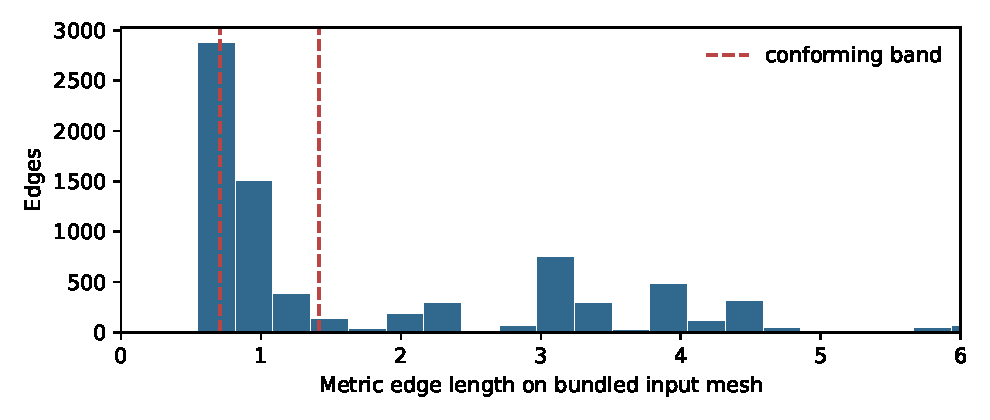
\includegraphics[width=.85\linewidth]{docs/figures/metric_edges.pdf}
\caption{Metric edge lengths on the bundled cube input, computed from its 1,241 points and 6,144 tetrahedra. The plot uses the endpoint-length logarithmic mean and counts each unique edge once.}
\label{fig:edges}
\end{figure}

\clearpage
\subsection{CAD boundary fidelity}
\texttt{tools/egads\_boundary\_fidelity.py} reports distances between a mesh boundary and a supplied STEP model. It needs pyEGADS. The output is a console report, so capture it outside the input tree if you need a record:
\begin{lstlisting}[language=bash]
python tools/egads_boundary_fidelity.py --geo cases/cube_egads/input/geometry/cube.geo --mesh cases/cube_egads/input/mesh/cube1241.vol --step cases/cube_egads/input/geometry/cube.step
\end{lstlisting}
Figure~\ref{fig:distance} shows point-to-CAD-face distance. The drawing is a schematic; its distances do not come from the cube case.
\begin{figure}[H]
\centering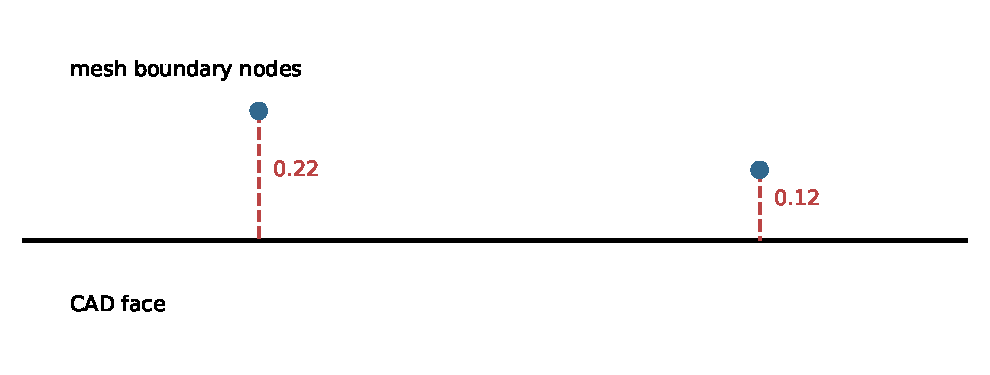
\includegraphics[width=.78\linewidth]{docs/figures/cad_distance_definition.pdf}
\caption{Schematic boundary-node distances to a CAD face. A fidelity report measures actual mesh and model coordinates; this drawing only shows the geometric quantity.}
\label{fig:distance}
\end{figure}

\subsection{Mesh conversion}
\texttt{tools/convert\_mesh.py} turns a Gmsh 2.2 ASCII bridge into Netgen \texttt{.vol}. The optional geometry file can reclassify boundary faces, and \texttt{--with-edges} writes ridge segments. Choose an output directory outside \texttt{input/}:
\begin{lstlisting}[language=bash]
python tools/convert_mesh.py /tmp/amac-cube-cross/bridge_0.msh bridge_0.vol --output-dir /tmp/amac-converted --geo cases/cube_cross/input/geometry/cube.geo --with-edges
\end{lstlisting}
A \texttt{.vol} without edge segments loses ridge and corner classification when read back. Preserve the original case inputs and compare surface IDs after conversion if your downstream solver depends on them.

\clearpage
\section{What the recorded results say}
Table~\ref{tab:results} reports conditioned historical results. A new run at this checkout may differ. The maximum-size cross metric in the last row is not one of the four bundled case files. Both runs used one process and four Numba threads on engine commit \texttt{4da7d28}, dated 2026-11-05. Both runs completed their stated iteration caps.

\begin{table}[H]
\centering\small
\begin{tabular}{p{.25\linewidth}rrrrr}
\toprule
Case and metric & Iter. & Tets & Conforming & Mean $Q$ & Flat\\
\midrule
Coarse cross, bundled metric & 12 & 2,696 & 89.44\% & 0.5400 & 0\\
Cross, $h_{\max}=0.125$ & 20 & 6,896 & 76.47\% & 0.2778 & 0\\
\bottomrule
\end{tabular}
\caption{Conditioned study results: one process, four threads, engine commit \texttt{4da7d28}, 2026-11-05. The coarse cross row uses the bundled \texttt{cube\_cross\_coarse} input; the maximum-size row uses a separate generated cross metric.}
\label{tab:results}
\end{table}

The maximum-size run had minimum $Q=2.690\times10^{-3}$, below the $0.01$ poor-element threshold, although it had no flat or inverted tets. Its mean $Q=0.2778$ misses the study target of $0.3$. The other eight historical 20-iteration sensitivity runs used an earlier engine state and were not repeated after the surface-label and reprojection fixes. Compare only runs with their case, metric, iteration cap, thread count, engine state and date recorded.

\section{Limits and troubleshooting}
AMAC needs an initial mesh and does not supply a curvature-aware metric. The CAD adapter accepts one STEP body. An uncertain face mapping warns but can proceed. A failed inverse evaluation can fall back without a counted adaptation total. Check a coarse curved boundary with the fidelity tool.

The analytical geometry reader recognizes planes and spheres. Other constructive solid geometry syntax does not add analytical projection support. A \texttt{.vol} bridge can lack edge segments; use the conversion tool's \texttt{--with-edges} option when downstream code needs ridge classification.

If activation cannot find TBB, rerun \texttt{bash setup.sh} and source \texttt{activate.sh} in a fresh shell. The engine expects Numba's TBB threading layer. Do not launch a run from an unrelated interpreter: inspect the Python path printed by activation and use \texttt{python} from that shell. If a conda environment is active, deactivate it before sourcing \texttt{activate.sh}; the script rejects that combination so its pinned environment stays unambiguous. If pyEGADS is absent, use the cube cross case or install optional ESP support for CAD.

When the driver says an input is missing, run \texttt{--check} and inspect the resolved path. Relative input paths start at the case directory, not the current shell directory. When it refuses output under \texttt{input/}, choose a sibling result directory. When it refuses an existing directory, use a fresh path or check the old results before passing \texttt{--force}. For a quality concern, inspect \texttt{adaptation\_history.json}, the full log and the final mesh; the terminal summary alone cannot show each rejected local move.

\clearpage
\section{References}
\begin{enumerate}[leftmargin=*]
\item Loseille and Alauzet (2011), continuous mesh framework and metric complexity.
\item Loseille and L\"ohner (2010), local cavity adaptation and quality gates.
\item Knupp (2001), algebraic tetrahedron quality.
\item Michal and Krakos (2012), metric edge length and tetrahedron quality equations.
\item Vlachos et al. (2001), PN triangles for the mesh-based curved-boundary fallback.
\item Balan, Park and Anderson, NASA Refine, for the adaptation cycle and comparison with an independent implementation.
\item Tavva, thesis Chapter 4, for the analytic cross and cylinder metric equations.
\end{enumerate}
\end{document}
